\documentclass[a4paper,12pt]{article}

\usepackage{alltt, fancyvrb, url}
\usepackage{graphicx}
\usepackage[utf8]{inputenc}
\usepackage{float}
\usepackage{hyperref}
\usepackage[italian]{babel}
\usepackage[table]{xcolor}
\usepackage{array}
\usepackage{multirow}
\usepackage{titlesec}
\usepackage{listings}
\usepackage[italian]{cleveref}
\usepackage{acronym}
\usepackage{subcaption}

\renewcommand{\thesection}{\arabic{section}}

\sloppy
\setlength{\parindent}{0pt}

\title{\textbf{Project Network Diagram}}
\author{}
\date{}

\begin{document}
\maketitle
\tableofcontents

\newpage

\section{Project Network Diagram}
Innanzitutto, abbiamo creato il \textit{Project Network Diagram}, nel quale sono state inserite tutte le attività
collegate in base alle dipendenze. Le dipendenze individuate sono di due tipi: \textit{Finish-to-Start (FS)} e
\textit{Finish-to-Finish (FF)}. \\
A partite dal diagramma abbiamo derivato il \textit{Gantt Chart}, mostrato in \cref{fig:gantt-chart}, dal quale si può
vedere anche il \textit{Critical Path}, composto dalle attività che nella figura sono colorate di rosso.
\footnote{\textit{Le attività sono state inserite con una durata di un giorno, ad eccezione delle attività 1.2.1 e
4.2.2 che erano state stimate precedentemente (riportate nel file \textit{estimations.pdf}).}}
Pertanto le attività non presenti nel percorso critico, hanno qualche giorno di \textit{slack}.
La parallelizzazione delle attività è possibile, ma limitata dalle risorse disponibili.

\begin{figure}[H]
    \centering
    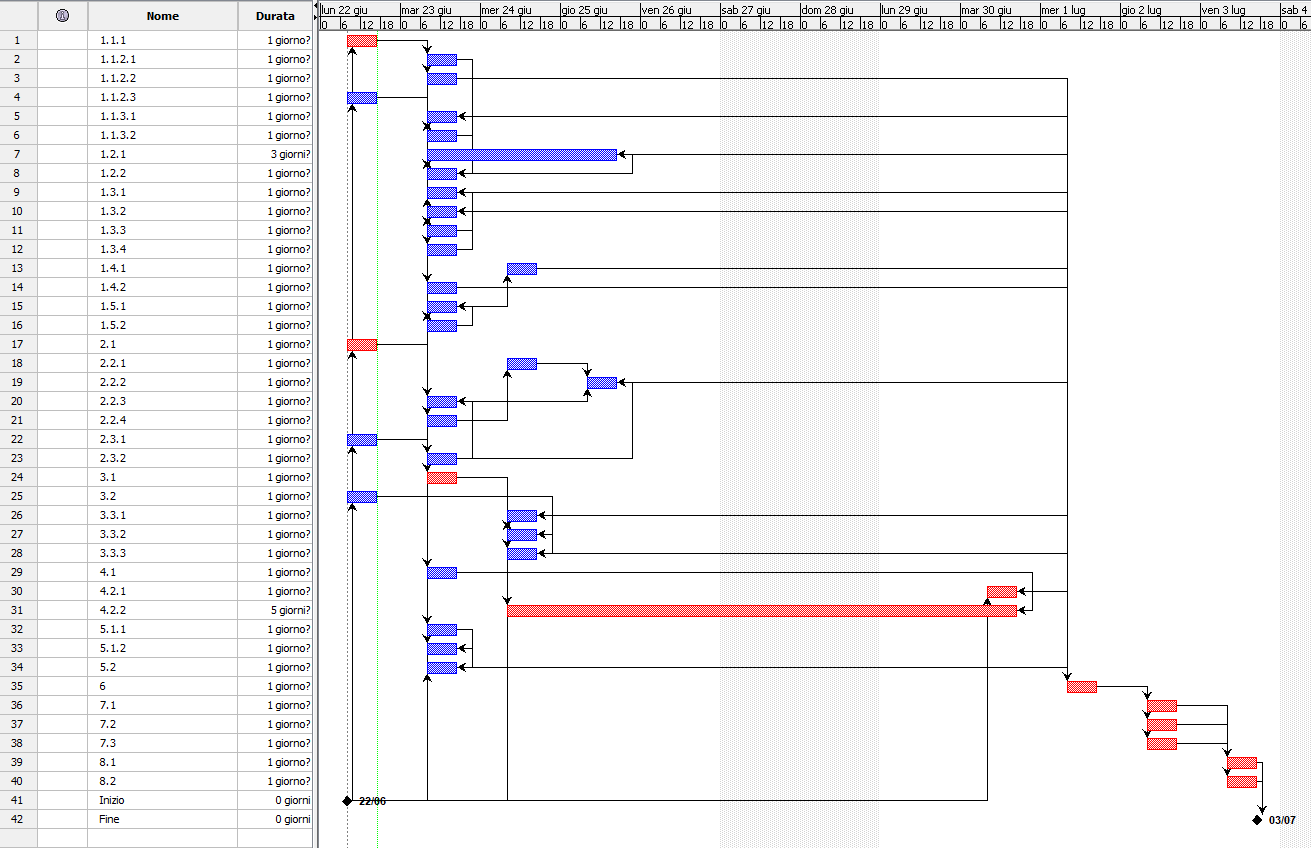
\includegraphics[width=\textwidth]{images/gantt.png}
    \caption{Gantt Chart}
    \label{fig:gantt-chart}
\end{figure}

\section{Milestones}
Sono state individuate due milestones intermedie, in relazione alla WBS:
\begin{itemize}
    \item \textbf{milestone 1:} completamento dei requisiti 1, 2 e 3;
    \item \textbf{milestone 2:} completamento dell'applicazione web (requisiti 4 e 5).
\end{itemize}
Le date di completamento delle due milestones e di fine progetto equivalgono alle date di completamento delle attività
stimate nel Gantt Chart.

\section{Analisi della schedula}
Data la stima di fine progetto e una \textit{scope bank} del 10\% della durata complessiva del progetto, non è
necessario comprimere la schedula, in quanto il progetto può essere completato entro i tempi richiesti.

\end{document}
